\chapter{Cloud Storage Services Comparison}\label{ch:cloud-storage-services-comparison}

\section{Introduction}
Cloud storage solutions are rapidly rising in popularity among individuals and enterprises, with the benefits of using such services in day-to-day life and business becoming more and more evident. Cloud storage applications like Google Drive are used by almost 40\% of households in certain areas while, by 2025, 100 \textit{Zettabytes} of data (50\% of all data) will be stored in the cloud~\cite{zeta}.

Customers nowadays have dozens of options when it comes to storage providers. Some of the most popular ones are established providers like Dropbox~\cite{dropbox}, and tech giants such as Amazon and Microsoft, that offer their \ac{s3}~\cite{s3} and Azure Blob services~\cite{blob}, respectively. All storage services, however, differ in certain characteristics like pricing, capacity and performance. It becomes important, then, to investigate these differences in order to make an educated decision on which service to adopt.

The first distinction that needs to be made is between cloud \textit{object} storage and cloud \textit{file} storage~\cite{objectvsfile, objectvsfile2,ibm_cloud_storage}:

\subsection{Object storage}
This technology allows data to be stored and managed in an unstructured format called \textit{objects}. Objects include the data that make up a file, user-created metadata and a unique identifier. They are stored in a flat data environment which enables fast scaling and application can easily retrieve objects of any data type, using the metadata, identifier, object contents and other properties.

As businesses expand, they are tasked with handling larger and larger volumes of data from a variety of sources that is used by both applications and users. This data is often unstructured and in many different formats and storage media, making it hard to store it in a central repository. Therefore, cloud object storage can solve this issue as it offers vast scalability and cost-efficient storage tiers for storing all kinds of data natively in a single virtual repository, accessible from anywhere and on a pay-as-you payment model. However, object storage also has some disadvantages. Specifically, the format which object storage uses is slower than other storage types. Additionally, an object cannot be modified after it is created, it must instead be overwritten. So, object storage is  ideal for large amounts of unstructured data that does not need to be read regularly. An example of cloud object storage is Amazon S3~\cite{s3}.

Some common use cases for object storage are:
\begin{itemize}
    \item[--] \textit{\textbf{Data lakes}}, which are centralized repositories for storing data of any scale, structured or unstructured, and rely on object storage to operate~\cite{datalake}. They offer encryption, access control and great scalability, allowing for easy and dynamic storage expansion of up to petabytes of content with a pay-as-you-go charging model.

    \item[--] The virtually limitless data that is stored in cloud object storage is often used by businesses to perform \textit{\textbf{big data analytics}}, in an effort to better understand their customers, operations and market.

    \item [--] Cloud object storage provide flexible data storage for \textit{\textbf{cloud-native applications}}, accessible via an API, thus aiding developers and allowing for easier and faster deployment.

    \item[--] An excellent use of object storage is \textbf{\textit{data archiving}}, replacing on-site archive infrastructure and providing enhanced data security, durability, accessibility and near-instant retrieval times.

    \item [--] Object storage systems can used to replicate data across many systems, regions and data centers, ensuring that \textbf{\textit{backups}} are ready to be used for recovery from hardware failures.

    \item [--] Replication on a global scale can be achieved with cloud object storage, vastly reducing the storage costs and increasing availability for \textit{\textbf{rich media}} like music, videos and digital images.

    \item [--]  Since \textit{\textbf{\ac{ml}}} models generate inferences after being trained over billions of data items, object storage becomes a necessity to handle such scale in a cost-efficient manner.
\end{itemize}

\subsection{File Storage}
In contrast to object storage, file storage utilizes a hierarchical structure for storing data, where files are stored inside of folders which are grouped into directories and so on, and strict protocols like \ac{nfs} are used. Consequently, it is more difficult to locate a specific piece of data among billions, compared to object storage, where each object is uniquely identified. In addition, the inherent hierarchy and pathing limits the potential scalability of cloud file storage, whereas object storage provides near-limitless scaling. Additionally, while unstructured data can be stored using file storage, it makes it much harder to work with such data, especially at large scales.

File synchronization is one of the major features that have contributed to the popularity of these systems. File storage allows users to automatically synchronize their files across a variety of devices, making it very convenient and simple to continue their work as they left it. Another popular use case of file storage collaborative work, as the most up-to-date version of a file can be easily shared among a group of users~\cite{personal1}. Furthermore, access rights and limits (e.g. write-only, password protection) can be set by the user on a per-file basis. The user interface and experience of cloud file storage services are also significantly more user-friendly and familiar, with many useful features for daily use such as file previews, making them suitable for casual and experienced users alike. An example of cloud file storage is Dropbox~\cite{dropbox}.


\section{Object Storage Services}
Two of the most popular object storage services are Amazon \ac{s3} and Microsoft Azure Blob Storage.

In Amazon S3, objects are stored in buckets, and prefixes (shared names) are used to organize objects. \textit{S3 object tags}, which are a set of up to 10 key-value pairs, can also be appended to objects to make storage management easier, as these tags can be added and edited at any point in the object's lifetime for stronger access control and other use cases. In addition, \textit{S3 inventory} reports can be generated manually or automatically to provide information on the objects in a bucket, to make working with lots of data easier and to allow gathering information on encryption, replication and more. Amazon provides an online Management Console, a \ac{rest} API, a \ac{cli} and an \ac{sdk} in various languages for accessing S3 features~\cite{s3faq}.

Microsoft Azure Blob Storage uses three types of related resources. The first are storage accounts, which provide a unique namespace for the user's data and is used in the address of each object. There are different kinds of storage accounts, each tailored for different uses and with different redundancy options~\cite{blobaccounts}:

\begin{enumerate}

    \item \textit{General-purpose v2} is the standard account for storing blobs (data). It is recommended for most use cases.

    \item \textit{Premium block blobs}, for block blobs and append blobs. Makes use of \ac{ssd} technology, making it ideal for workloads that require low latency or that involve many transactions.

    \item \textit{Premium page blob}, which is similar to a premium block bob account, but it's only used for page blobs.

\end{enumerate}

Containers are the second resource, which organize a set of blobs. An unlimited number of containers can be included in a storage account, and an unlimited number of blobs can be stored in a container. The third and final resource kind are blobs, of which there are three types:

\begin{enumerate}
    \item \textit{Block blobs} are made up of blocks of data, with each block being uniquely identified. Block blobs are ideal for large amounts of text or binary data, as up to 50.000 variable size blocks can be included in a single block blob.

    \item \textit{Append blocks} are also made up of blocks of data, but they are optimized for append operations, making them ideal for use cases like \ac{vm} data logging.

    \item \textit{Page blobs}  are composed of 512-byte pages and are suitable for random write and read operations. They support Azure virtual machines by acting as disks.
\end{enumerate}

As with S3, to help the management of large pools of data, Blob storage provides the ability to use \textbf{blob index tags}, key-value pairs that can be used to categorize blobs, find specific blobs across an entire account, set permissions and more. With \textbf{Azure Cognitive Search}, blob contents are imported as search documents that are indexed, allowing for the information stored in the blob data themselves to be searched. Also, with the help of \ac{ai} enrichment, text from images can be extracted. Furthermore,  \textbf{Blob inventory} automatically generates report with user-defined rules to provide an overview on containers, snapshots, blobs, blob versions and their properties. Blob storage object are accessible via REST API, Azure PowerShell (cmdlets of Azure resources)~\cite{powershell}, CLI or a client library in one of many languages.~\cite{blobinfo}

Both S3 and Blob Storage also provide\textbf{ monitoring and logging} for their resources to keep track of their performance, operation, cost efficiency and security and to receive alerts for specified events. S3 has automatic (Cloudwatch Alarms and Cloudtrail Log Monitoring) and manual (S3 dashboard, AWS Trusted advisor and more) monitoring tools, while logging is possible via server access logs (for object-level operations) and API call logs with AWS CloudTrail (for bucket-level and object-level visibility). Azure Blob Storage works with Azure Monitoring (used for all Azure resources) for monitoring and logging purposes.~\cite{s3monitoring,blobmonitoring} In addition, S3 offers even further enhanced storage visibility via S3 Storage Lens and S3 Storage Class Analysis. The former provides a single view of storage usage and activity patterns across potentially thousands of accounts at various levels and provides actionable recommendations for improving data protection and cost efficiency. At the same time, Storage Class Analysis helps in making the correct storage class transitions by monitoring object access patterns.~\cite{s3analytics}

\subsection{Storage Classes}
Blob Storage and S3 both offer various storage classes to match the data access patterns and resiliency requirements of different workloads, at the lowest cost possible.

S3 makes the following distinctions regarding its storage classes: ~\cite{s3faq}
\begin{description}
    \item[S3 Standard] is recommended by Amazon for regularly accessed data, offering great performance, availability and durability for data that is regularly accessed. It is characterized by high throughput and low (millisecond) latency, making it ideal for big data analytic, gaming applications, content distribution and many more scenarios. In general, S3 classes allows the customers to make configurations at the object level, and a bucket can contain objects stored across different classes.

    \item [S3 Standard-Infrequent Access (S3 Standard-IA)] is best used for less frequently accessed data, that nonetheless must be rapidly accessed when required. It is identical to standard S3 in terms of latency, throughput and durability, but with low price (in GB storage) and retrieval, meaning that it is suitable for data to be stored long-term, for disaster recovery files and for backups.

    \item[S3 One Zone-Infrequent Access (S3 One Zone-IA)] is identical to S3 Standard-IA, with the difference being that data is stored in one \ac{az}, instead of three like the other storage classes. This has the immediate effect of 20\% lowers costs, but if the single AZ is destroyed, all data will be lost along with it.

    \item[S3 Glacier] classes are tailor-made for archiving purposes, and there are three of them:
    \begin{itemize}
        \item [--] \textit{S3 Glacier Instant Retrieval} offers the lowest cost for storing data long-term which is rarely accessed and need to be retrieved in millisecond. If the data is accessed once every 4 months, around 70\% will be saved in storage costs when compared with S3 Standard-IA. This class is the fastest in accessing archived data, whilst having the same throughput performance and access latency as S3-standard, meaning that it is ideal for medical images, news media content and more data which is archived but need instant access.

        \item[--] \textit{S3 Glacier Flexible Retrieval}, which formerly was S3 Glacier, offers 10\% lower, compared to Glacier Instant Retrieval, costs for archived that is to be accessed once or twice per year and do not require immediate access. It balances costs and access times (can be from hours or minutes), making it ideal for use cases like disaster recovery and backups.

        \item[--] \textit{S3 Glacier Deep Archive} offers the lowest storage costs in Amazon S3, used for retaining and preserving data long-term, which might be accessed 1 or 2 times per year. It offers retrieval times of up to 12 hours, and targets customers that need to retain data for many years to meet regulations, making it especially applicable for healthcare, public sector and other industries. It can also replace magnetic tape systems.
    \end{itemize}

    \item[S3 Intelligent-Tiering] automatically moves data to the access tier such that the costs will be minimized, with no impact in terms of performance, retrieval costs or operation. It charges a small fee every month for monitoring and automatically moving objects, but can lead to immense cost savings. If an object hasn't been accessed for 30 or 90 days, it is moved automatically to the Infrequent and Archive Instant Access tier, respectively. If the user does not require immediate retrieval, an object can be automatically moved to the deep Archive Tier after not being accessed for 180 days. Of course, if an object in one of these tiers is accessed, then it reverts to the frequently accessed tiers, but objects in Deep Archive first need to be restored (three options exists for archive retrieval, with different access times for each).~\cite{archiverestore} This class is ideal for data with access patterns that are not known or that are unstable.

    \item[S3 Outposts] provides on-premise objects storage, which is useful for data that needs to be stored locally to meet performance, processing or residency requirements, while also taking advantage of S3 features offered on the cloud, as the same APIs are used.
\end{description}

S3 also provides object\textbf{ Lifecycle management}, which allows for defining an object's lifecycle with a policy to automatically migrate objects from the S3 standard class to others, thus saving on storage costs and accommodating different access patterns. Most transitions between classes are supported, but there are exceptions because, for instance, an object can't be transitioned to S3 standard from any other class. Furthermore,  policies can be set to automatically remove objects and incomplete multipart uploads according to their age, which saves in storage costs and time. Lifecycle rules allow for great configuration, as they can be used in conjunction with prefixes to, for example, discard specific objects after a certain number of days has passed.~\cite{s3lifecycle}

\bigskip
Blob Storage offers its own access tiers: ~\cite{blobinfo}
\begin{description}
    \item[Hot Tier] is used for storing data online that is actively used or that will be accessed regularly. It is the costliest for storing data, but the cheapest for accessing it.

    \item[Cool Tier] also stores data online, but the data is to be accessed less frequently (short-term backups are example use cases). This tier has the same access latency, durability, and throughout performance as the hot tier, but slightly lower availability. It also has higher access costs, but lower storage costs overall, hence why it is ideal for data that isn't very frequently used.

    \item[Archive Tier] is the offline tier offered by Blob Storage, ideal for storing data that is only rarely accessed. It offers the lowest overall storage costs, but higher latency and retrieval costs when compared to the online tiers. This tier is suitable for scenarios like long-term backups and archival data which is very infrequently accessed. However, it must be mentioned that, depending on redundancy configurations, not all accounts are allowed to move blobs to the archive tier and archived blobs cannot be read or modified, so they must be first rehydrated from the Archive tier. Rehydration is possible by either changing the blob's access tier to either hot or cold, or by copying it to one of those tiers. The time required for rehydration depends on the priority, as standard priority rehydration may take 15 hours for objects of under 10 GB in size, whereas high priority rehydration could complete in under an hour.
\end{description}

Changing a blob's access tier is possible by manually setting the blob tier or by copying the blob to another tier. The former is recommended as it avoids the early deletion penalty which, in the case of cold tier blobs, incurs a charge if a blob is deleted or moved to a different tier less than 30 days after being created. S3 also has a similar penalty for its classes. Like S3, Blob Storage allows for \textbf{Lifecycle Management}, providing the opportunity to set cost-efficient policies with rules that specify when data should be transitioned to another tier, according to access patterns, and when objects should be expired, according to age.

\subsection{Data Redundancy}
Amazon Simple Storage Service strengthens data redundancy thanks to \textbf{S3 Replication}, for which 3 different options exist: ~\cite{s3replication}
\begin{itemize}
    \item [--] \textit{S3 \ac{crr}} can be used to replicate along with their tag and metadata to other AWS regions. This helps with compliance requirements for storing data at great distances, latency minimization by maintaining data close to customers, disaster recovery and more.

    \item [--] \textit{S3 \ac{srr}} replicates data between buckets, but only within the same region. Example use cases include aggregating data (e.g. logs) in a single location for processing or abiding by legal requirements that require data to be kept in another AWS account in the same region.

    \item [--] \textit{S3 Batch Replication} is unique as it replicates existing objects, instead of newly created ones like CRR and SRR do. So, it complements the other replication methods and can be used for instance to reattempt failed replications or to migrate existing objects to other buckets.
\end{itemize}

Another S3 feature is \textbf{Replication Time Control}, which is backed by an \ac{sla} and claims that, during any month, 99.99\% of objects will be replicated within 15 minutes, otherwise Service Credits will be provided to the customer as compensation.~\cite{s3replicationsla}

S3 allows replication to happen at a bucket level, a shared prefix level or an object level (using object tags) with multiple destination buckets in the same or different regions and even two-way replication among buckets is possible. On top of all this, \textbf{S3 Multi-Region Access Points} can vastly boost performance (up to 60\%) as it automatically routes requests to the copy with the lower latency, taking into account location,  network congestion etc. It can be used in unison with CRR to allow for a single endpoint for all replicas, hence simplifying management ~\cite{s3replication}.

According to Amazon, S3 storage classes (except Outposts and S3 One Zone-IA) redundantly store data across 3 AZs (at least), thus attaining 11 9's (99.99999999999\%) of objects durability for a given year, meaning that with 10 million objects stored, one will be lost every 10 thousand years. S3 Outposts enforce durability by redundantly storing data across devices within the on-premises data center, while S3 One Zone-IA does the same but within a single AZ.

\bigskip
In the primary region, Azure Blob always replicate data three times and 2 redundancy options are provided: ~\cite{blobinfo}
\begin{itemize}
    \item [--] \textit{\ac{lrs}} synchronously copies data in a primary region data center. It is the cheapest but least durable option (at least 11 9s), as if some sort of disaster occurs in the data center all copies will be lost. It could be useful for abiding to requirements that restring data to only a single region, or for data that can be easily reconstructed after loss.

    \item[--] \textit{\ac{zrs}} also synchronously replicates data in the primary region, but across different Azure availability zones (physical locations), hence attaining at least 12 9's of storage durability, so it is a better choice for high durability requirements, although region-wide disasters might still lead to data loss.
\end{itemize}

Microsoft also allows and recommends replicating data to a secondary region far from the primary region in order to survive regional disasters. There exist two options for secondary region redundancy:
\begin{itemize}
    \item [--]  \textit{\ac{grs}} first uses LRS for the primary region, and then asynchronously replicates the data in a secondary region , where again LRS is used. It claims significantly higher durability (at least 16 9's) during a year.

    \item [--] \textit{\ac{gzrs}} is the most robust replication option. It is identical to GRS, with the only (significant) difference being that ZRS is used initially, instead of LRS. This results in the combined benefits of both high availability in the primary zone (ZRS) and protection against a regional disaster (geo-replication). It provides 16 9's of durability or more yearly.
\end{itemize}
It should be noted that data stored in secondary regions is normally only accessible after an outage renders the primary region unavailable, and the asynchronous replication leads to the secondary region being slightly outdated. The option, however, exists to allow reading data in the secondary region via the \ac{ra-grs} or \ac{ra-gzrs} configurations.

\subsection{Availability}
With the S3 SLA, a commitment is made by Amazon to maintain a specific uptime percentage for its services every month~\cite{s3sla}. If lower than promised availability for a service is observed during a month (exceptions apply for unusual situations like natural disasters), then customers are entitled to Service Credits which can be applied against future payments towards that service. The percentage of charges for a billing cycle that service credits cover is based on \autoref{S3 SLA}.

\begin{table}[h]
	\centering
	\caption{S3 Availability SLA}
	\label{S3 SLA}
	\begin{tabular}{|c|c|c|}
		\hline
		\rowcolor[HTML]{EFEFEF} 
		\textbf{Service Credit} &
		\textbf{\begin{tabular}[c]{@{}l@{}}Standard/ Glacier/\\ Glacier Deep Archive\end{tabular}} &
		\textbf{\begin{tabular}[c]{@{}l@{}}Intelligent-Tiering/ Standard-IA/\\ One Zone-IA/ Glacier Instant Retrieval\end{tabular}} \\ \hline
		10\%  & \textless{}99.9\% and \textgreater{}= 99\% uptime & \textless{}99\% and \textgreater{}= 98\% uptime \\ \hline
		25\%  & \textless{}99\% and \textgreater{}= 95\% uptime   & \textless{}98\% and \textgreater{}= 95\% uptime \\ \hline
		100\% & \textless{}95\% uptime                            & \textless{}95\% uptime                          \\ \hline
	\end{tabular}
\end{table}

Blob Storage also provides an availability SLA~\cite{blobsla}, again offering credits as compensation for lower-than-expected uptime.(\autoref{Blob SLA})
\begin{table}[h]
	\centering
	\caption{Blob Storage Availability SLA}
	\label{Blob SLA}
	\resizebox{\textwidth}{!}{
	\begin{tabular}{|c|c|c|c|}
		\hline
		\rowcolor[HTML]{EFEFEF} 
		\textbf{Service Credit} &
		\textbf{Hot Blobs} &
		\textbf{Cool Blobs} &
		{\color[HTML]{333333} \textbf{Archive Blobs}} \\ \hline
		10\% &
		\begin{tabular}[c]{@{}c@{}}\textless{}99.9\% write requests \\ in LRS, ZRS, GRS, RA-GRS\\ \\ \textless{}99.99\% read requests \\ in RA-GRS\end{tabular} &
		\begin{tabular}[c]{@{}c@{}}\textless{}99\% write requests\\  in LRS, GRS, RA-GRS\\ \\ \textless{}99.9\% read requests\\  in RA-GRS\end{tabular} &
		\begin{tabular}[c]{@{}c@{}}\textless{}99\% write requests \\ in LRS, GRS, RA-GRS\\ \\ \textless{}99.9\% read requests \\ in RA-GRS\end{tabular} \\ \hline
		25\% &
		\begin{tabular}[c]{@{}c@{}}\textless{}99\% write requests \\ in LRS, ZRS, GRS, RA-GRS\\ \\ \textless{}99\% read requests\\  in RA-GRS\end{tabular} &
		\begin{tabular}[c]{@{}c@{}}\textless{}98\% write requests \\ in LRS, GRS, RA-GRS\\ \\ \textless{}98\% read requests \\ in RA-GRS\end{tabular} &
		\begin{tabular}[c]{@{}c@{}}\textless{}98\% write requests \\ in LRS, GRS, RA-GRS\\ \\ \textless{}98\% read requests \\ in RA-GRS\end{tabular} \\ \hline
	\end{tabular}}
\end{table}

\subsection{Security}
S3 and Blob Storage both follow strict security standards and they offer lots of support for access control and encryption.

\subsubsection{Data Handling}
For securing \textbf{data in transit}, Amazon recommends using HTTPS (TLS) to prevent eavesdropping , man-in-the-middle and other attacks. Conditions can be set on bucket policies so that only encrypted connections (over HTTPS) are allowed, and a rule can be used to check that all buckets require \ac{ssl} to be used by requests. Client-side encryption is also allowed, which can be achieved in one of two ways: ~\cite{s3securitypractices,s3clientside,s3vsblobsecurity}

\begin{enumerate}
    \item Using a AWS \ac{kms} key ID, clients can request a unique data key to encrypt an object before uploading it. AWS KMS then sends a plaintext version of the key and its cipher blob which will be included in the object metadata. To download an object, the client downloads the cipher blob and the encrypted object, and then sends the blob to AWS KMS to get the plaintext data key for decryption.

    \item Clients can also generate, use and store their own encryption keys (called root keys), which will be provided to the S3 encryption client to generate and encrypt a one-time symmetric encryption key (data key) that will encrypt the uploaded object. Object metadata is used to determine the root key that will decrypt the data key for a downloaded object. So, it is up to the client here to manage the keys and encryption process, but they can decide what root keys to use (e.g. symmetric), the algorithms etc.
\end{enumerate}

In similar fashion, Blob Storage has the option of requiring API calls to be made over HTTPS and clients can even enforce a minimum TLS version for incoming requests, enhancing overall security. Furthermore, client-side encryption can also be used, which works similarly as it does in S3, the main difference being that encryption keys can be stored either locally or on the Azure Key Vault, which is Azure's personal key management solution.~\cite{blob_minimum_tls,blob_clientside,azure_vault,blob_secure_transfer}

\textbf{Data at rest} can be protected in S3 using client-side encryption (as described earlier) and server-side encryption, and there are three mutually-exclusive options for the latter: ~\cite{s3serverside}

\begin{itemize}
    \item [--] With \textit{\ac{sse-s3}}, each object is encrypted with a unique key which itself is encrypted with a root key that changes frequently. All this is handled by S3. A very strong 256-bit block cipher is used for encryption.

    \item [--] \textit{\ac{sse-kms}} is identical to SSE-S3, but has the added protection that comes with the separate access permissions involving KMS keys, and provides an audit trail for these keys. SSE-KMS allows the keys to be handled and generated by the user or Amazon S3, and some extra fees are applied.

    \item [--] \textit{\ac{sse-c}} is also similar, but the customer is responsible for providing and securely storing the encryption key, with Amazon handling the encryption/decryption processes.
\end{itemize}

Blob Storage also allows client- and server-side encryption for data at rest, and for the latter it uses strong 256-bit encryption,which is automatically enabled for all storage accounts and access tiers. Encryptions are typically managed by Microsoft, however users can manage their own keys in either (or both) of the following two ways: ~\cite{blob_at_rest,blob_keys1,blob_keys2}

\begin{itemize}
    \item [--] \textit{Customer-managed keys}, which can be stored using some of Azure's key management solutions (e.g. Azure Vault), and they can be created by the customer or by the Azure Key Vault APIs.

    \item [--] \textit{Customer-provided keys}, which are encryption keys that the client provides on requests to Blob storage. This key is discarded as soon as the operation completes, and the same key must be used for subsequent operations on that blob.
\end{itemize}

A unique feature of Azure Storage is the option for \textit{double encryption}, which involves encryption at both service and infrastructure levels, with different keys and algorithms. This protects against potential compromises of algorithms or keys, making it ideal for customers that require higher security for their data. For encryption at the infrastructure level, the keys are always managed by Microsoft.~\cite{blob_at_rest} However, using Azure Storage Accounts also involves the security of two 512-bit storage account keys which are used for authorizing access to data in the account. Microsoft heavily emphasizes their importance and recommends using Azure Key Vault for their management and frequent rotation (instead of manual management), and urges customers to never distribute them or store them anywhere where they can be easily accessed.~ \cite {blob_account_keys}

\subsubsection{Access Control}
To control access to its resources, S3 employs many mechanisms, which include: ~\cite{s3faq, s3_access,s3_access_guidelines,s3_scp,s3_vpc,s3vsblobsecurity}

\begin{description}
    \item[\ac{iam}] can be used to manage the access that users have to S3 resources. IAM users, groups and roles can be created, and policies can be attached to them specifying the level of access they have to any resource. Extra security can be added with \ac{mfa}, requiring for example a code generated by a software app in addition to regular credentials.

    \item[\ac{acl}] are examples of resource-based policies, since they are attached to the S3 resources. Each resource (bucket, object) has an ACL attached to it which lists what AWS accounts have what permissions. Some restrictions do exist, for example permission can only be granted to other AWS accounts, and Amazon actually recommends disabling ACLs and instead simplifying management by automatically having the bucket owner also own all objects in the bucket (regardless of whoever uploaded it). Instead, ACL should only be used for specific cases where individual access to each object needs to be configured.

    \item[Bucket policies] also are resource-based policies that can be added by the bucket owner, specifying the permissions that other AWS accounts and IAM users have for accessing bucket contents. Bucket policies can replace ACL, and they are necessary for cross-account permissions as ACL doesn't cover every permission, while user policies are only for users in the same account as the bucket.

    \item[\ac{scp}] allow control over the maximum permissions for all organizational accounts. They are supplementary as they do not actually set permissions, but merely set limits that all accounts must follow to stay within organizational guidelines.

    \item[S3 Block Public Access] provides a centralized way for controlling public access to resources, overriding any potential change to permissions that users may have made, hence strengthening security.

    \item[Query String Authentication] involves the creation of a limited-time URL for accessing an object.

    \item [\ac{vpc}] enable the launch of resources into a virtual network that the customer defines, and VPC endpoints are VPC entities which can offer direct (without internet) connectivity to S3. Access to S3 data can then be controlled by either controlling the users, groups etc. that can use an endpoint, or by controlling which endpoints can access the buckets (using bucket policies).
\end{description}

Along with S3, Blob Storage offers its own range of options for authorizing data access: ~\cite{blob_authorization,blob_endpoint}

\begin{description}
    \item[A Shared Key] could be used by a client, passing a timestamp and authorization header with every request. This method is not recommended, and users are urged to disable it.

    \item[\ac{sas}] involve the use of a limited-time signed URL which grants controlled access to resources.

    \item[Azure \ac{ad}] is the recommended authorization method by Microsoft, providing centralized, secure and easy access control for resources across many Azure services. Azure \ac{rbac} can be used to manage a user's, group's etc. access to blobs by assigning them a role, while \ac{abac} builds on this to add conditions to these roles. Azure AD also supports MFA and passwordless authentication.

    \item[Anonymous public read access] can be toggled on to allows data to be read without authorization but it can also be disallowed, in which case authorization becomes mandatory.

    \item[Private endpoints] can additionally be used, so that traffic between clients and the storage account goes through Microsoft's network and not through the public internet.
\end{description}


\subsection{Data Protection}
To protect data from accidental deletions or modifications, and to recover from any such accidents, S3 uses the following mechanisms: ~\cite{s3faq}

\begin{enumerate}
    \item \textit{Versioning}, once enabled for a bucket, preserves all object versions and allows for easy recovery from accidental deletions and overwrites, by rolling back to any previous version. Versioning can be used in conjunction with S3 lifecycle rules to maintain a rollback window for objects and, for example, store older object versions in a cheaper storage class and automatically delete them after a specified time period has elapsed. This cuts down on costs while also providing a recovery window to previous versions. For even further data protection, MFA Delete can be enabled to add another layer of security, requiring MFA on top of account credentials in order to permanently delete an object version.

    \item \textit{S3 Object Lock} prevents object version deletion and overwrite until a specified amount of time has passed, or until a legal hold is lifted, regardless of storage class or lifecycle transitions used. Object Lock can be enabled at the bucket or object level, and helps in complying with regulations enforcing  \ac{worm} data protection.
\end{enumerate}


Azure Blob also provides comparable data protection options: ~\cite{blob_data_protection}

\begin{enumerate}
    \item \textit{Storage account locks} can prevent accounts from being deleted (CannotDelete lock)  and their configurations from being modified (ReadOnly lock)

    \item \textit{Immutability policies} can be applied to data, maintaining them in a WORM state for a specified interval or until a legal hold is removed. Immutability policies can be applied at the version-level, but only after a default policy has been configured at the account- or container-level. Immutability policies can also be applied at the container-level, in which case the same policy applies for all objects in that container.

    \item \textit{Soft delete} retains blobs or containers that have been deleted or overwritten for a specified time period, after which the deletion is permanent.

    \item \textit{Blob versioning} maintains previous states (versions) of a blob, which can be used for recovery purposes.  \textit{Point-in-time restore} is similar to versioning, but is only used for block blobs. A cheaper alternative is \textit{blob snapshots}, which allow users to manually saving states when needed, hence cutting down on costs, however \textit{snapshots }are deleted when the objects themselves are deleted.
\end{enumerate}

\subsection{Performance}
Regarding performance, Microsoft has published some performance targets for Blob storage.~\cite{blob_targets} While they are high-end, these targets can be achieved keeping in mind that the observed performance always depends on various factors like workload type, object size and more. Some key performance targets are shown in \autoref{Blob targets}

\begin{table}[h]
	\caption{\label{Blob targets}Blob Storage Performance Targets}
    \resizebox{\textwidth}{!}{%
        \begin{tabular}{|l|l|}
            \hline
            \rowcolor[HTML]{EFEFEF} 
            \multicolumn{1}{|c|}{\textbf{Resource}}                   & \multicolumn{1}{c|}{\textbf{Target}}                     \\ \hline
            Maximum container size                                       & Same as maximum storage account capacity (default 5 PiB) \\ \hline
            \multicolumn{1}{|c|}{Maximum number of blobs and containers} & Unlimited                                                \\ \hline
            Maximum block blob size                                      & 50,000 X 4000 MiB ($\sim$190 TiB)                        \\ \hline
            Blob request rate                                            & Up to 500 requests per second                            \\ \hline
            Maximum blob size via PUT operation                          & 5000 MiB                                                 \\ \hline
            Maximum ingress in LRS/GRS/ZRS regions                       & 60 Gbps                                                  \\ \hline
            Maximum egress in LRS/GRS/ZRS regions                        & 120 Gbps                                                 \\ \hline
            Maximum ingress in other regions                             & 25 Gbps                                                  \\ \hline
            Maximum egress in other regions                              & 50 Gbps                                                  \\ \hline
        \end{tabular}%
    }
\end{table}

Amazon hasn't made any performance targets publicly available, however the maximum size of an object can range from 0 bytes up to 5 TB. A single PUT operation, meanwhile, can upload an object that is 5GB in size at most. Furthermore, the maximum number of buckets in an account is 100 by default, and this limit can be increased to 1000 by paying a service fee. There is no maximum bucket size limit.~\cite{s3faq, s3_limits}

The work done in~\cite{s3vsblob_performance} sheds more light on the performance of cloud storage solutions including S3, S3 Glacier, Blob Storage, as various generated workloads (differing in file size and number) were used to measure and compare the actual performance of each service during 2013-2014.

\subsubsection{Latency}
The authors in \cite{s3vsblob_performance} calculated the \ac{rtt} experienced when using cloud storage services, as shown in \autoref{fig:latency}
\begin{figure} [h]
    \centering
    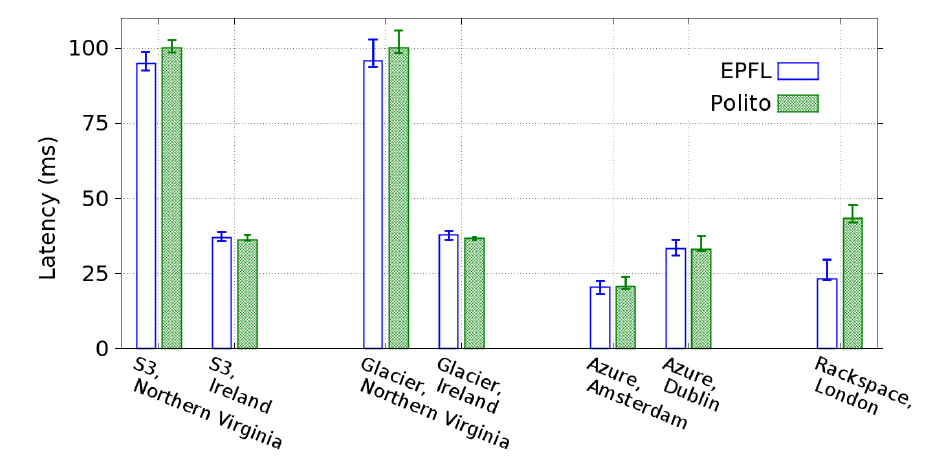
\includegraphics[scale=0.7]{images/latency}
    \caption{\label{fig:latency}Latency of cloud services}
\end{figure}


It was established from the results that RTTs are stable and nearly identical for S3 and Azure services (in the same regions), and the determining factor was propagation delay (due to distance from data center).

\subsubsection{Throughput}
Research was also conducted in \cite{s3vsblob_performance} to measure throughput when downloading single files and bundle of files. Results are in \autoref{fig:throughput} .
\begin{figure} [h]
    \centering
    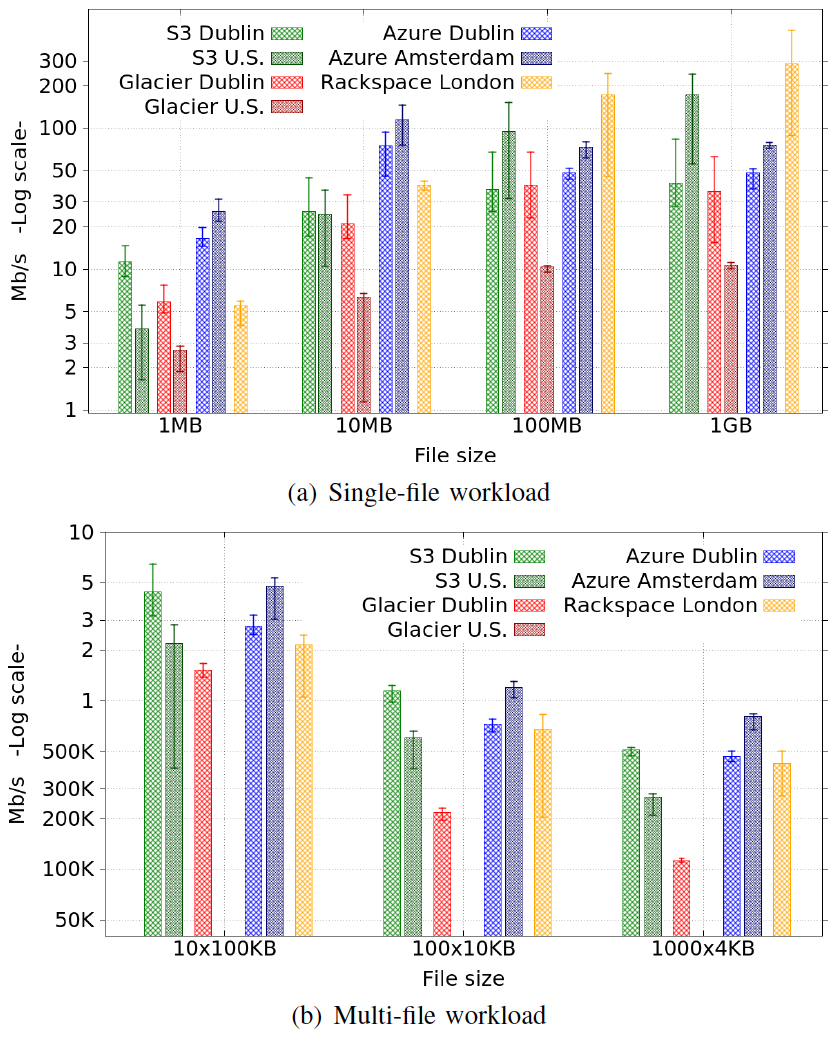
\includegraphics[scale=0.5]{images/throughput}
    \caption{\label{fig:throughput}Download throughput of cloud services}
\end{figure}

Across all services, performance improves for large files but this is a natural result of \ac{tcp} algorithms. Glacier is by far the slowest service (with strict download limits set), which is natural as it is meant for archiving. In general, however, there is no clear winner as Azure performs better for small files, while S3 comes on top for large files, and there also exist performance differences for each service's data centers, which is probably a result of differences in connection quality. In addition,  the results are similar when it comes to downloading bundles of files, though overall throughput is vastly reduced due to the overhead involved in managing the vast number of files .

\subsubsection{Performance Variation}
Another benchmark in \cite{s3vsblob_performance} was carried out to determine if the performance of each services varies due to, for example peak traffic causing slowdown at certain points in the day.
\begin{figure} [h]
    \centering
    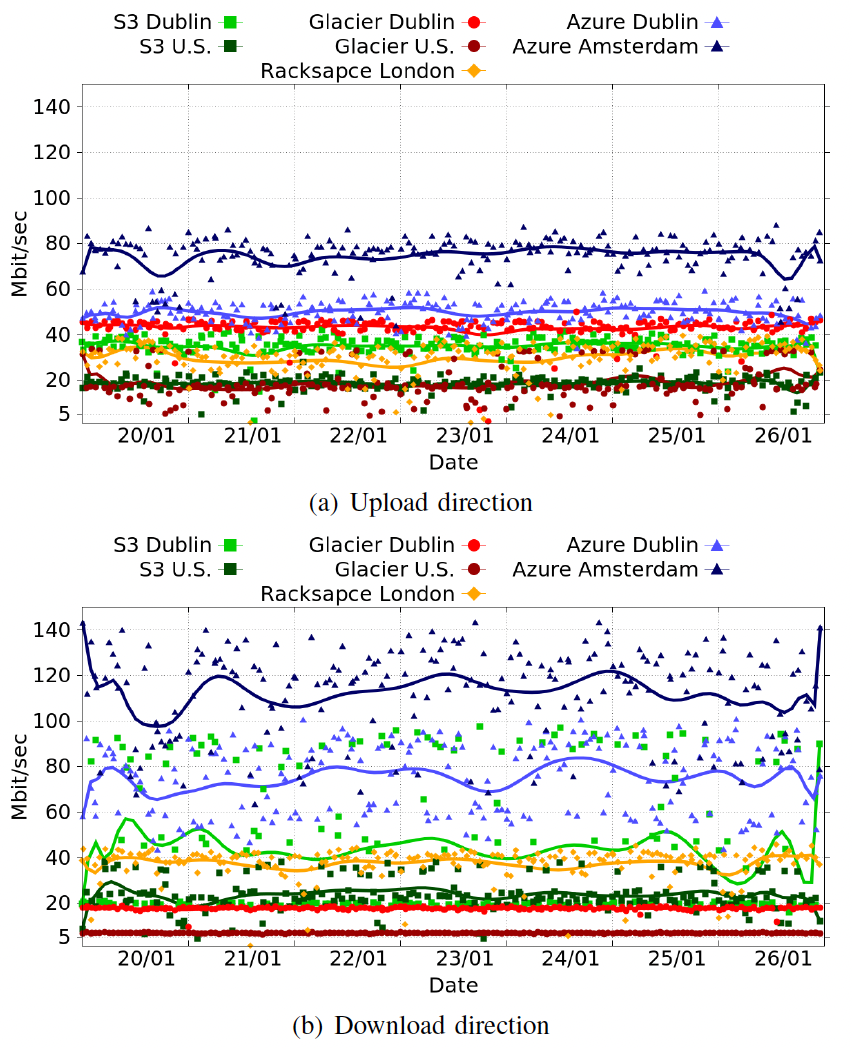
\includegraphics[scale=0.5]{images/variation}
    \caption{\label{fig:variation}Performance variation of cloud services}
\end{figure}

As shown in \autoref{fig:variation}, upload speeds remain almost perfectly stable across all providers. Download speeds, on the other hand, vary wildly depending on the service, data center and workload. Glacier speeds remain capped as mentioned earlier, while Azure performs the best (likely due to the small workload size). S3 in Dublin shows the greatest variation, frequently jumping between 20 and 100 Mb/s, due to the great difference in performance capability of the server group that is reached each time (one is limited to 20 Mb/s).

\subsubsection{Connection Management and Overhead}
The way each service manages its connection when uploading multiple files also affects the amount of overhead that is generated each time. Amazon offers the most cleverly implemented services in this regard, since S3 uses two connections, one for user login and another for data transfer, while Glacier uses only a single connection for both (regardless of the number of uploaded files). Azure, however, uses a separate connection for each transferred file, and so it suffers from especially increased overhead when many small files are uploaded. (\autoref{fig:overhead})

\begin{figure} [h]
    \centering
    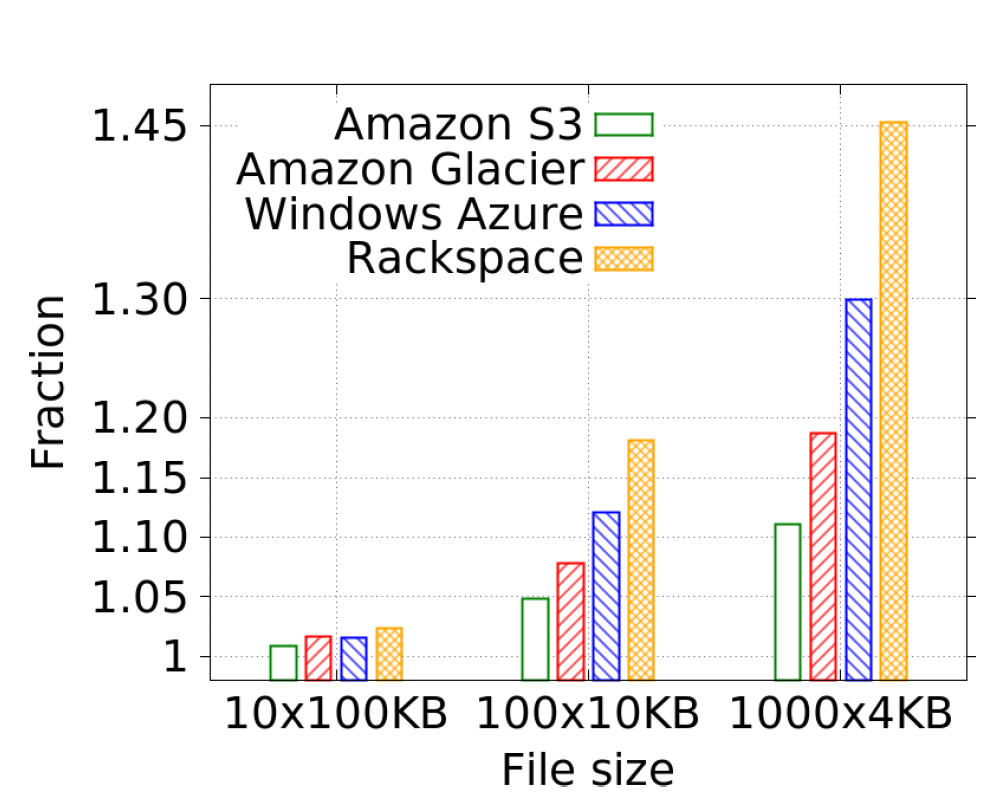
\includegraphics[scale=0.3]{images/overhead}
    \caption{\label{fig:overhead}Upload overhead of cloud services}
\end{figure}

\subsection{Pricing}
Azure Blob and S3 both are based on a "pay-as-you-go" charging model,  and the results for some comparable storage classes are shown below. The prices shown in \autoref{tab:object_pricing} are for the US East (N.Virginia) S3 region and East US 2 Blob region. Blob Storage also takes into account the redundancy method used when presenting the prices and, for Blob, the flat structure namespace option was selected~\cite{s3_pricing,blob_pricing}.

\begin{table}[!h]
    \resizebox{\textwidth}{!}{%
        \begin{tabular}{|llll|}
            \hline
            \multicolumn{1}{|l|}{} &
            \multicolumn{1}{l|}{\textbf{Amazon S3-IA}} &
            \multicolumn{1}{l|}{\textbf{Blob Cool Tier LRS}} &
            \textbf{Blob Cool Tier GRS} \\ \hline
            \multicolumn{4}{|c|}{\cellcolor[HTML]{EFEFEF}\textbf{Data Storage}} \\ \hline
            \multicolumn{1}{|l|}{Per Month Storage} &
            \multicolumn{1}{l|}{\$0.0125 per GB} &
            \multicolumn{1}{l|}{\$0.01 per GB} &
            \$0.02 per GB \\ \hline
            \multicolumn{4}{|c|}{\cellcolor[HTML]{EFEFEF}\textbf{Data Transfer}} \\ \hline
            \multicolumn{1}{|l|}{Data Retrieval} &
            \multicolumn{1}{l|}{\$0.01 per GB} &
            \multicolumn{1}{l|}{\$0.01 per GB} &
            \$0.01 per GB \\ \hline
            \multicolumn{1}{|l|}{Transfer IN from Internet} &
            \multicolumn{1}{l|}{Free} &
            \multicolumn{1}{l|}{Free} &
            Free \\ \hline
            \multicolumn{1}{|l|}{Transfer TO another Region/AZ} &
            \multicolumn{1}{l|}{$0.01 - $0.02 per GB} &
            \multicolumn{1}{l|}{\$0.01 per GB} &
            \$0.01 per GB \\ \hline
            \multicolumn{4}{|c|}{\cellcolor[HTML]{EFEFEF}\textbf{Requests}} \\ \hline
            \multicolumn{1}{|l|}{Write Requests} & \multicolumn{1}{l|}{\$0.01 per 1,000 requests}  & \multicolumn{1}{l|}{\$0.1 per 10,000 requests}   & \$0.2 per 10,000 requests   \\ \hline
            \multicolumn{1}{|l|}{Read Requests}  & \multicolumn{1}{l|}{\$0.001 per 1,000 requests} & \multicolumn{1}{l|}{\$0.01 per 10,000 requests}  & \$0,01 per 10,000 requests  \\ \hline
            \multicolumn{1}{|l|}{Delete} &
            \multicolumn{1}{l|}{Free} &
            \multicolumn{1}{l|}{Free} &
            Free \\ \hline
            \multicolumn{1}{|l|}{Other Requests} & \multicolumn{1}{l|}{\$0.001 per 1,000 requests} & \multicolumn{1}{l|}{\$0.004 per 10,000 requests} & \$0.004 per 10,000 requests \\ \hline
        \end{tabular}%
    }\caption{\label{tab:object_pricing}Object Storage Pricing Sample}
\end{table}

It can be observed from ~\autoref{tab:object_pricing} that, in general, S3 and Blob prices are similar, with Blob Cool Tier LRS overall being a bit cheaper than S3-IA, and GRS being the most expensive of the three. However, this is only a sample, and the cost-efficiency of each service can only be determined after extensive analysis and careful consideration of various factors like the storage classes and redundancy options selected, workloads to be carried out and more.

One interesting discovery was made in~\cite{s3vsblob_performance}, which was that, while S3's expected charges are more or less identical to actual charges, Blob's actual charges in bandwidth and storage are 25\% cheaper than expected.

\section{File Storage Services}
In this section, a comparison will be made between three popular File Storage Services, namely Dropbox, Google Drive and Box.

\subsection{Pricing Plans and Scalability}
All 3 services offer a variety of pricing plans ~\cite{dropbox,google_drive,box}, and the primary examples of each are summarized in tables  \autoref{tab:Dropbox_Pricing}, \autoref{tab:Box_Pricing}, and \autoref{tab:Drive_Pricing}.

All 3 providers also offer a free plan with significant limitations, for instance Box's free plan (Individual) includes 10 GB of storage and 1 version per file only, while Drive's personal plan includes 15 GB storage per user while limiting sharing capabilities. Furthermore, all providers unlock more storage and features (especially regarding security and management) as more expensive plans are chosen.

Out of the 3, Box offers the most expensive plans, with Enterprise being almost double the price of the other providers' costliest plans. However, Box does offer unlimited storage for most of its plans, though, unlike the other two which impose a limit on at least one of these metrics in most of their plans.  By far the most cost-effective plans, though, are offered by Google Drive, as all plans include every application that is part of Google Workspace. This means that along with Drive, customers get access to email, video conference, chatting and other applications. All providers also offer custom plans, the specifics of which (e.g. price, storage) are determined after contacting the sales team.

In terms of \textbf{scalability}, all 3 services are comparable, supporting most file types along with unlimited users, devices and storage capacity. The main difference can be seen in the upload file size limit, with Google Drive being the most scalable with a 5 TB limit (although there is a 750GB daily upload limit)  and Dropbox falling a bit behind at 2 TB, while Box is significantly limited at 150 GB per file.


\begin{table}[]
    \resizebox{\textwidth}{!}{%
        \begin{tabular}{|l|c|c|c|c|c|}
            \hline
            & \cellcolor[HTML]{EFEFEF}\textbf{Plus} & \cellcolor[HTML]{EFEFEF}\textbf{Family} & \cellcolor[HTML]{EFEFEF}\textbf{Professional} & \cellcolor[HTML]{EFEFEF}\textbf{Standard} & \cellcolor[HTML]{EFEFEF}\textbf{Advanced} \\ \hline
            \textbf{\begin{tabular}[c]{@{}l@{}}Price (billed annually)\\ per month\end{tabular}} & 9.99€ & 16.99€ & 16.58€ & 12€ per user & 18€ per user \\ \hline
            \textbf{Storage} & 2,000 GB & 2,000 GB & 3,000 GB & 5,000 GB & \begin{tabular}[c]{@{}c@{}}As much as needed,\\ after purchase\end{tabular} \\ \hline
            \textbf{File upload size limit} & 2 TB & 2 TB & 2 TB & 2 TB & 2 TB \\ \hline
            \textbf{Users} & 1 user & 6 users & 1 user & 3+ users & 3+ users \\ \hline
            \textbf{Dropbox Sign} & Yes & Yes & Yes & Yes & Yes \\ \hline
            \textbf{Dropbox Backup} & Yes & Yes & Yes & Yes & Yes \\ \hline
            \textbf{\begin{tabular}[c]{@{}l@{}}File recovery \\ and versioning\end{tabular}} & 30 days & 30 days & 180 days & 180 days & 1 year \\ \hline
            \textbf{Dropbox Rewind} & 30-day history & 30-day history & 180-day history & 180-day history & 1-year history \\ \hline
            \textbf{\begin{tabular}[c]{@{}l@{}}Shared link \\ controls\end{tabular}} &  &  & Yes & Yes & Yes \\ \hline
            \textbf{\begin{tabular}[c]{@{}l@{}}External sharing \\ controls\end{tabular}} &  &  &  & Yes & Yes \\ \hline
            \textbf{\begin{tabular}[c]{@{}l@{}}Ransomware detection\\ and recovery\end{tabular}} &  &  &  &  & Yes \\ \hline
            \textbf{Security alerts} &  &  &  &  & Yes \\ \hline
            \textbf{Dropbox Passwords} & Yes & Yes & Yes & Yes & Yes \\ \hline
            \textbf{Dropbox Vault} & Yes & Yes & Yes &  &  \\ \hline
            \textbf{MFA} & Yes & Yes & Yes & Yes & Yes \\ \hline
            \textbf{Dropbox Capture} & \begin{tabular}[c]{@{}c@{}}120 mins and \\ HD quality\end{tabular} & \begin{tabular}[c]{@{}c@{}}120 mins and\\ HD quality\end{tabular} & \begin{tabular}[c]{@{}c@{}}Unlimited time,\\ 4K quality and\\ video editing\end{tabular} & \begin{tabular}[c]{@{}c@{}}Unlimited time,\\ 4K quality and\\ video editing\end{tabular} & \begin{tabular}[c]{@{}c@{}}Unlimited time,\\ 4K quality and\\ video editing\end{tabular} \\ \hline
            \textbf{Dropbox Transfer} & Up to 2 GB & Up to 2 GB & Up to 100 GB & Up to 2 GB & Up to 100 GB \\ \hline
            \textbf{File locking} &  &  & Yes & Yes & Yes \\ \hline
            \textbf{Full text search} & Yes & Yes & Yes & Yes & Yes \\ \hline
            \textbf{\begin{tabular}[c]{@{}l@{}}Admin console and\\ multi-team login\end{tabular}} &  &  &  & Yes & Yes \\ \hline
            \textbf{\begin{tabular}[c]{@{}l@{}}Single sign-on\\ (SSO)\end{tabular}} &  &  &  &  & Yes \\ \hline
            \textbf{Email and chat support} & Yes & Yes & Yes & Yes & Yes \\ \hline
            \textbf{\begin{tabular}[c]{@{}l@{}}Phone support during\\ business hours\end{tabular}} &  &  &  & Yes & Yes \\ \hline
        \end{tabular}%
    }
    \caption{Dropbox Pricing}
    \label{tab:Dropbox_Pricing}
\end{table}

\begin{table}[]
    \resizebox{\textwidth}{!}{%
        \begin{tabular}{|l|c|c|c|c|c|}
            \hline
            & \cellcolor[HTML]{EFEFEF}\textbf{Business Starter} & \cellcolor[HTML]{EFEFEF}\textbf{Business} & \cellcolor[HTML]{EFEFEF}\textbf{Business Plus} & \cellcolor[HTML]{EFEFEF}\textbf{Enterprise} & \multicolumn{1}{l|}{\cellcolor[HTML]{EFEFEF}\textbf{Enterprise Plus}} \\ \hline
            \textbf{\begin{tabular}[c]{@{}l@{}}Price (billed annually)\\ per month\end{tabular}} & 4.50€ & 13.50 per user€ & 22.50€ per user & 31.50€ per user & Custom \\ \hline
            \textbf{Storage} & 100 GB & Unlimited & Unlimited & Unlimited & Unlimited \\ \hline
            \textbf{Upload file size limit} & 2 GB & 5 GB & 15 GB & 50 GB & 150 GB \\ \hline
            \textbf{Users} & 3-10 users & 3+ users & 3+ users & 3+ users & Unlimited \\ \hline
            \textbf{Box Sign} & 10 signatures & Unlimited Signatures & Unlimited Signatures & Unlimited Signatures & Unlimited Signatures \\ \hline
            \textbf{\begin{tabular}[c]{@{}l@{}}File recovery \\ and versioning\end{tabular}} & 25-version history & 50-version history & 50-version history & 100-version history & Unlimited \\ \hline
            \textbf{\begin{tabular}[c]{@{}l@{}}Sharing permissions\\ and controls\end{tabular}} & Yes & Yes & Yes & Yes & Yes \\ \hline
            \textbf{Box Shield} &  &  &  & Yes & Yes \\ \hline
            \textbf{\begin{tabular}[c]{@{}l@{}}User and security\\ reporting\end{tabular}} &  & Yes & Yes & Yes & Yes \\ \hline
            \textbf{Box Keysafe} &  &  & Yes & Yes & Yes \\ \hline
            \textbf{MFA} & Yes & Yes & Yes & Yes &  \\ \hline
            \textbf{\begin{tabular}[c]{@{}l@{}}Advanced Search \\ Filters\end{tabular}} &  & Yes & Yes & Yes & Yes \\ \hline
            \textbf{\begin{tabular}[c]{@{}l@{}}Admin console and\\ role delegation\end{tabular}} &  &  & Yes & Yes & Yes \\ \hline
            \textbf{\begin{tabular}[c]{@{}l@{}}Single sign-on\\ (SSO)\end{tabular}} &  & Yes & Yes & Yes & Yes \\ \hline
            \textbf{Customer support} & Business hours & Business hours & Business hours & Business hours & 24/7/365 Support \\ \hline
        \end{tabular}%
    }
    \caption{Box Pricing}
    \label{tab:Box_Pricing}
\end{table}

\begin{table}[!b]
    \resizebox{\textwidth}{!}{%
        \begin{tabular}{|l|c|c|c|c|}
            \hline
            & \cellcolor[HTML]{EFEFEF}\textbf{Business Starter} & \cellcolor[HTML]{EFEFEF}\textbf{Business Standard} & \cellcolor[HTML]{EFEFEF}\textbf{Business Plus} & \cellcolor[HTML]{EFEFEF}\textbf{Enterprise} \\ \hline
            \textbf{Price per month} & \$6 per user & \$12 per user & \$18 per user & Custom \\ \hline
            \textbf{Storage} & 30 GB per user & 2 TB per user & 5 TB per user & As much as needed \\ \hline
            \textbf{File upload size limit} & 30 GB & 2 TB & 5 TB & 5 TB \\ \hline
            \textbf{Users} & 30 users & 30 users & 30 user & Unlimited users \\ \hline
            \textbf{\begin{tabular}[c]{@{}l@{}}File recovery \\ and versioning\end{tabular}} & \begin{tabular}[c]{@{}c@{}}30 days and\\ 100 versions\end{tabular} & \begin{tabular}[c]{@{}c@{}}30 days and\\ 100 versions\end{tabular} & \begin{tabular}[c]{@{}c@{}}30 days and\\ 100 versions\end{tabular} & \begin{tabular}[c]{@{}c@{}}30 days and\\ 100 versions\end{tabular} \\ \hline
            \textbf{Shared drives} &  & Yes & Yes & Yes \\ \hline
            \textbf{Target audience sharing} &  & Yes & Yes & Yes \\ \hline
            \textbf{\begin{tabular}[c]{@{}l@{}}Ransomware, malware\\ and spam detection\end{tabular}} & Yes & Yes & Yes & Yes \\ \hline
            \textbf{Security alerts} &  &  &  &  \\ \hline
            \textbf{Google Vault} &  &  & Yes & Yes \\ \hline
            \textbf{MFA} & Yes & Yes & Yes & Yes \\ \hline
            \textbf{File locking} & Yes & Yes & Yes & Yes \\ \hline
            \textbf{Google Cloud Search} &  & 1st party data & 1st party data & \begin{tabular}[c]{@{}c@{}}1st and 3rd\\ party data\end{tabular} \\ \hline
            \textbf{\begin{tabular}[c]{@{}l@{}}Group-based \\ policy controls\end{tabular}} & Yes & Yes & Yes & Yes \\ \hline
            \textbf{\begin{tabular}[c]{@{}l@{}}Single sign-on\\ (SSO)\end{tabular}} & Yes & Yes & Yes & Yes \\ \hline
            \textbf{Security center} &  &  &  & Yes \\ \hline
            \textbf{Customer support} & Standard support & Standard support & Standard support & Enhanced support \\ \hline
        \end{tabular}%
    }
    \caption{Google Drive Pricing}
    \label{tab:Drive_Pricing}
\end{table}

\subsection{File Sharing}
One of the primary reasons that people make use of cloud file storage services is the ability to easily share content among large groups of people, while keeping the content up-to date for everyone.

\textit{Dropbox} allows exactly this, as files (and folders) of any size (up to the maximum storage space) can be shared with anyone, regardless of Dropbox membership, by just providing them a link. It is also possible to create groups of people, and then invite them at once to access any shared files. The sender is notified of any changes made to shared files and by whom, while granular file or folder permissions can be applied to control exactly who can see which files and who can make what changes (edit, comment or just view file) or share content. To further enhance security, an expiration date and password can be set and downloads can be disabled for shared links.  Other useful features are file requests for collecting files from others even if they don't have a Dropbox account and  \textbf{Dropbox Transfer}, which is optimal for sending large files  (up to 250 GB) since sharing is possible without these files taking up storage space~\cite{dropbox}.

\textit{Box} also facilitates the sharing of files and folders by allowing the creation of shared links. These links can be used to send files of any size (up to the account limit) to others so that everyone has access to the latest version of a file, and recipients need not have a Box account. File transfer is made secure with the existence of 7 different permission levels for content, link expiration and download restrictions, while Box additionally allows file request links to be sent when files need to be gathered from many people (Box users or not)~\cite{box}.

The file sharing features of \textit{Google Drive} are similar, as customized (in terms of access control, expiration policy, recipients etc.) shared links to files (of any size) or folders can be created. However, Google Drive places some limits on the total number of people a file/folder can be shared with. for instance, only 50.000 individuals in total can have access to a shared file~\cite{google_drive,drive_sharing_limits}.

\subsection{Collaboration and Productivity}
Real-time collaboration is made easy with \textbf{Dropbox Paper}, Dropbox's own collaboration platform which offers a centralized place to carry out work on team projects. All types of content (e.g. notes, images, to-do lists, PDFs, GIFs etc. ) can be shared with team members who can contribute and leave feedback in real-time. Almost all file types can be easily previewed, relieving users of the need to download them, and annotations are possible directly on files, including PDFs (with Adobe Acrobat integration) and videos (with frame accuracy). Task management also becomes easier through Paper by assigning tasks with due date and reminders and by making use of tools that provide a bird's eye view on everyone's tasks and contributions. Furthermore, since Dropbox seamlessly integrates with many popular applications, members can keep using the tools they like and ,for instance, send files through Gmail or send messages to Microsoft Teams, without changing applications. On top of all this, Dropbox has its own video and screen capturing tools, document scanner (with \ac{ocr}) and eSignature tool (to easily sign any shared document and to gather signatures faster)~\cite{dropbox,dropbox_requests}.

\textbf{Box Notes} is Box's collaboration solution, that similarly offers a single place where videos, presentations and more can be shared and concurrently worked on by many editors. Files can be previewed directly and comments can be made, though only on text and image files, while tasks with due dates can be assigned and progress can be monitored to simplify task management. A unique feature is \textbf{Box Relay}, which automates and speeds up repeatable tasks (e.g. content reviews) by setting workflow triggers and outcomes. Additionally, Box's integration with more than 1.500 apps is seamless as, for instance, Box content can be directly accessed from Zoom or Slack. Like Dropbox, electronic signature, screen and video capturing solutions are also offered by Box~\cite{box,box_annotations}.

Drive supports collaboration by seamlessly integrating with the other apps that are part of Google Workspace. Specifically, \textbf{Google Docs} can be used to work with others on a single text document, making concurrent edits  and comments as needed (with spell-checking, which is missing from the other two providers) while painlessly connecting with other Google apps (e.g. Google Sheets and Slides for inserting spreadsheet data and slideshows,  Keep for making notes), and even Google Meet to directly join a meeting. Docs also facilitates task management, as to-do lists with deadlines can be created directly or through Google Tasks. However, Docs lacks significantly when it comes to previewing and annotating embedded media, and even embedding content from other Google apps is relatively cumbersome (no drag\&drop of files is supported).  Drive also has a document scanning functionality and integration with hundreds of 3rd-party apps is possible, like DocuSign for e-signatures and lucid charts for diagram creation~\cite{google_drive,google_docs,google_apps}.

\subsection{Security and Administration}
To enhance data protection, Dropbox applies encryption both in transit and at rest. For data transfer, SSL/TLS is used to create a secure tunnel protected by 128-bit or higher \ac{aes} encryption and files at rest are encrypted using 256-bit AES. To recover from unwanted modifications or deletions, permanent file deletes can be limited by admins, while file versions up to a year old can be recovered~\cite{dropbox_security}. This latter concept is taken even further with \textbf{Dropbox Rewind}, which allows reversing all content changes of the past year (at the folder- or account-level), making it ideal for recovering from scenarios like major data losses~\cite{dropbox_rewind}. Furthermore, \textbf{Dropbox Vault} is a PIN-protected folder, adding an extra layer of security for the most critical data. Regarding access management, \ac{sso} and two-step verification are offered, while each user can have both a personal and a work Dropbox to separate data for personal use from business data. Dropbox \ac{emm} allows teams to work with third-party EMM providers and control how members are using the Dropbox mobile app, by restricting its usage to select devices, tracking app usage (e.g. storage used and access locations) and remotely wiping devices~\cite{dropbox_emm}. Great control is given to Dropbox Business admins (who are assigned tiered roles) as they can manage users, track and terminate web sessions, unlink devices, configure centralized billing (by giving each employee their own Business account and paying for everything at once), reset passwords per-team or per-user and much more.  Admins can also gain in-depth visibility by generating comprehensive audit logs that include information on hundreds of filterable events including password changes, login attempts, file modifications, sharing events etc. and configurable alerts are triggered automatically when suspicious events occur~\cite{dropbox_admin}. By enabling automatic data classification, Dropbox can search for and label personal information to then provide admins with \ac{dlp} alerts when this content is shared externally~\cite{dropbox_dlp}. Finally, the always-on ransomware detection can alert admins via email when potential ransomware is identified, providing insight on the type and extent of the infection and recommending actions that should be taken (e.g determine alert validity and suspend affected members)~\cite{dropbox_ransomware,dropbox}.

Box's data encryption is comparable to Dropbox's, using TLS for data in transit and 256-bit AES encryption for data at rest, and even allowing users to manage and use their own encryption keys by leveraging AWS's Key Management Service with \textbf{Box KeySafe}. Versioning is also enabled, and the option is there for users to maintain all previous file versions if they so desire. User access is managed via MFA and SSO, and admins have granular control over passwords and can configure when sessions timeout. In addition, \textbf{Box Device Trust}  assists a company to meet their security policies by defining minimum OS version, encryption, antivirus and other requirements that devices need to fulfill before accessing Box, while device pinning sets a limit on the number of linked devices. Significant emphasis is given to mobile security, which is controlled by various settings that specify, for instance, if the device can save, print or upload content or if an application-specific passcode is required. Box further enhances mobile security by integrating with EMM providers which allows actions like restricting device access and checking app configurations before allowing access to Box content.~\cite{box_mobile,box_emm}. A unique Box feature is \textbf{Box Zones}, which helps with country- and region-specific data protection and privacy compliance requirements by allowing customers to decide which data to store in which region(s), with little setup time, automatic and non-intrusive migration of content and at no additional cost. In terms of admin controls, Box's \textbf{Admin Console} makes management simple as it can be used to easily manage users and their permissions, files, folders and many security settings (e.g. 2FA, password requirements). The Admin Console additionally  allows for extensive reports to be generated (manually or on a schedule), giving administrators full visibility on various topics including shared links, security events and user activity~\cite{box_admin}. Yet another useful security tool is \textbf{Box Shield}, which allows for automatic and manual classification of data using classification labels for which specific access policies can be defined, hence ensuring strong protection of the most critical data. At the same time, Shield scans all content (when updated, edited, deleted etc.) using its deep learning-based malware detection and also generates detailed timely security alerts when suspicious activity occurs that indicates compromised accounts or other potential security risks~\cite{box}.

Google Drive encrypts all files uploaded or created using AES 256-bit encryption, both in transit and at rest, but client-side encryption can also be used (with customer keys), for an added layer of encryption~\cite{drive_encryption,drive_client-side}. Using the native protection against malware, spam and ransomware, files can be proactively scanned and  automatically removed if any danger is identified. Additionally, file versions are maintained so that users can revert to them if they wish, but only the last 100 versions that are not more than 30 days old are maintained.  In general, Drive makes use of all the security features offered as part of Google Workspace. Specifically, a variety of login controls are available for Drive, including 2FA, SSO and web session length limit, while \textbf{Context-Aware Access} defines policies for accessing Drive based on device location, OS, if the device is company-owned etc.~\cite{drive_login_security,drive_context-aware}. There is also the ability for customers to select a geographic location for their data, however only two regions are available as options: Europe or the US, so this cannot help all companies meet their data residency requirements~\cite{drive_regions}. With \textbf{Google Endpoint Management}, both mobile and computer devices can be managed with the aim of making the data shared among them more secure. It allows for controlling which devices can access data, remotely sign out users or wipe devices, enforce strong passwords and device encryption and more. All these aforementioned controls are available to admins  through the \textbf{Admin Console}, via which users, user groups and shared folders are managed and various audit logs can be examined. Some use case for these logs are tracking how users collaborate and how much Drive storage they use, and assessing organizational security by checking for any data breaches or if anyone has installed 3rd party apps. Furthermore, admins are alerted about any potential security issues that arise, each of which is described and classified, while rules can be created to, among other uses, generate custom alerts and use DLP for sensitive data~\cite{drive_admin,drive_rules}. The Admin Console's advanced settings are expanded by the \textbf{Security Center} which offers three tools, the first being the security dashboard which provides an overview of various security reports that cover DLP incidents, suspicious attachments found, suspicious logins and more. The security center also offers the  investigation tool that allows accessing a log of devices used and their data, investigating file activity, take action on alerts etc. The third and last tool is the security health page, through which centralized controls for security settings of all user groups are available to the admin, along with recommendations for improving overall security~\cite{google_drive,drive_security_center}.

\subsection{Performance}
Extensive research into the performance of almost a dozen file storage services was carried out in~\cite{personal1}, where the authors introduced a methodology involving repeatable and automatically generated workloads of varying size and content to compare these services in terms of their capabilities, system design and data center locations, as well as to benchmark their performance on various metrics like synchronization delay, download speed and more.

\subsubsection{Capabilities}
Through the results gathered in~\cite{personal1}, it was confirmed that all tested cloud services use HTTPS to encrypt packets (HTTP is used only for Dropbox's notification protocols). Furthermore, to optimize network usage and transfer time, some specific client capabilities are used by all services:

\begin{description}
    \item[\textbf{Bundling}] involves gathering a batch of files in a bundle before transferring them, with the aim of reducing overhead and latency. From the 3 services discussed in this paper, both Box and Google Drive open several TCP connections during the submission of multiple files (with likely significant overhead) , as shown in  \autoref{fig:bundling},indicating that each file is managed separately. Dropbox, on the other hand, uses bundling as it opens only a few TCP connections for multiple files.

    \begin{figure} [h]
        \centering
        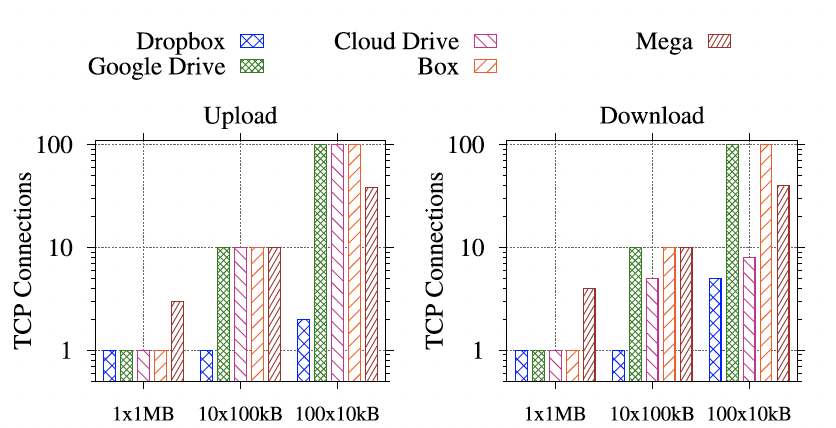
\includegraphics[scale=0.7]{images/bundling}
        \caption{\label{fig:bundling}Bundling capabilities}
    \end{figure}

    \item[\textbf{Chunking}] means transmitting large files in chunks, rather than in one transmission, simplifying error recovery and making partial submissions easier to implement. The TCP connections illustrated in \autoref{fig:chunking} reveal the chunking strategies used by Google Drive and Dropbox. Specifically, the former uses 8 MB chunks and the latter 4 MB chunks and, surprisingly, chunking is only used by Google Drive when downloading files. Additionally, while Box makes use of chunking~\cite{box_chunked}, the results on it from this experiment are not displayed.

    \begin{figure} [h]
        \centering
        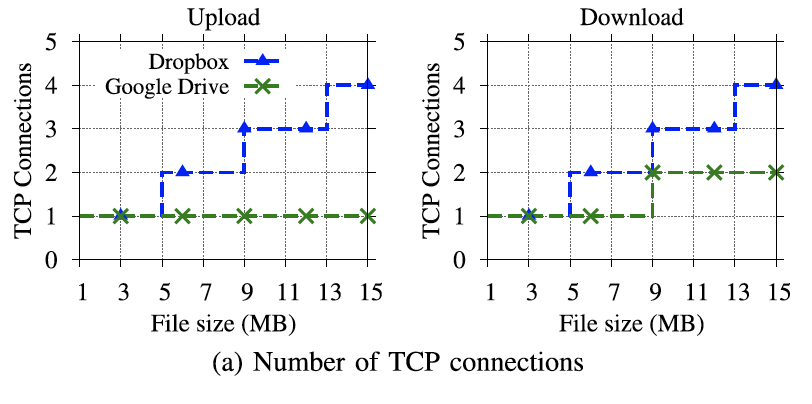
\includegraphics[scale=0.7]{images/chunking}
        \caption{\label{fig:chunking}Chunking capabilities}
    \end{figure}

    \item[\textbf{Compression}] of data helps with reducing network traffic and storage requirements and is used by Dropbox and Google Drive, with the latter's implementation being more efficient and smart since already compressed files (like JPEG) are not compressed a second time.

    \item[\textbf{Client-Side Deduplication}] can save upload capacity by identifying if the file already exists in the server. This identification is accomplished by first sending a file digest (calculated using the file's content) to the server, which checks if the file already exists to skip the upload.  Only Dropbox has deduplication capabilities, and copies of a file are identified even after they are deleted and subsequently restored.

    \item[\textbf{Delta Encoding}] allows the transmission of only the modified parts of a file, by calculating the differences between file versions, making it an attractive feature when files are frequently modified-e.g., for collaboration.  In \autoref{fig:delta encoding}, the effects of delta encoding when content is appended or inserted at random positions are shown, and it becomes obvious that only Dropbox uses delta encoding and, most of the time, only the modified content is uploaded. However, due to chunking, when a file is larger than the 4 MB chunk size, inserting content could then affect more than one chunk and thus lead to more data being transmitted.

        \begin{figure} [h]
        \centering
        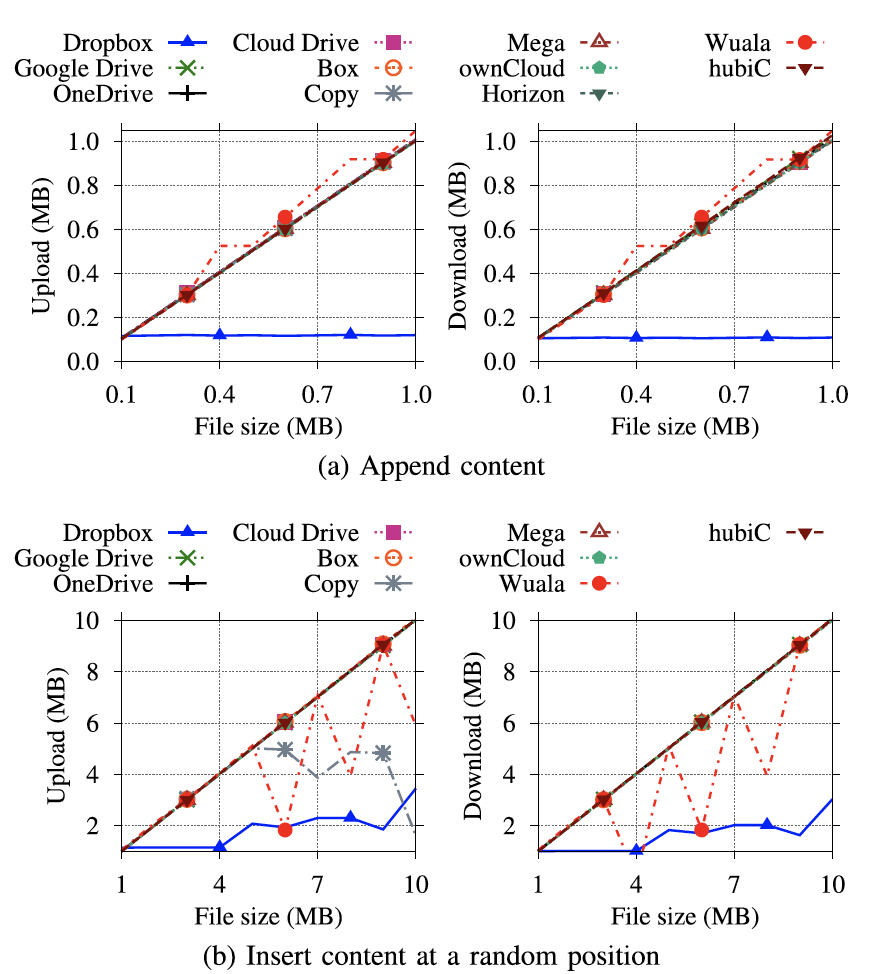
\includegraphics[scale=0.7]{images/delta_encoding}
        \caption{\label{fig:delta encoding}Delta encoding capabilities}
    \end{figure}

    \item[\textbf{\ac{p2p} Synchronization}] is only used by Dropbox, allowing for devices that host common files to synchronize among themselves without using the cloud which reduces internet and network traffic.
\end{description}

\subsubsection{Idle traffic and Data Center Placements}
Regarding the traffic generated while the cloud services are idle,~\cite{personal1} concluded that Dropbox, Box and Google Drive all generate negligible background traffic while idle, both during and after login.

When it comes to data center placements, Box allows users to store their data in a region of their choice thanks to Box Zones~\cite{box}, while Dropbox primarily stores data in the US but provides the ability to some business users for storing their data in the EU, Japan or the UK~\cite{dropbox_data_centers}. On the other hand, Google Drive uses a fully distributed topology, with more than 30 edge nodes spread across 6 continents. Using DNS load-balancing, clients are directed to the nearest edge node where TCP connections are terminated and traffic is routed to the data centers by making use of Google's private network. This, of course, has the net gain of smaller RTT and less overall traffic being offloaded from the public internet.

\subsubsection{Benchmarks}

The work carried out in~\cite{personal1} led to the following conclusions:

\begin{description}
    \item[\textbf{Synchronization Start Up}], or the amount of time required before synchronization starts, is depicted in \autoref{fig:synchronization start up}, where the empirical \ac{cdf} is obtained by considering 20 repetitions. Dropbox is the fastest for single small files, but it does experience delays when synchronizing multiple files due to bundling, in which case there is no clear winner. The CDF curves of Google Drive and Box, however, do present knees in this and other metric (as shown later), likely due to variability in traffic shaping or performance of their servers.

    \begin{figure} [h]
        \centering
        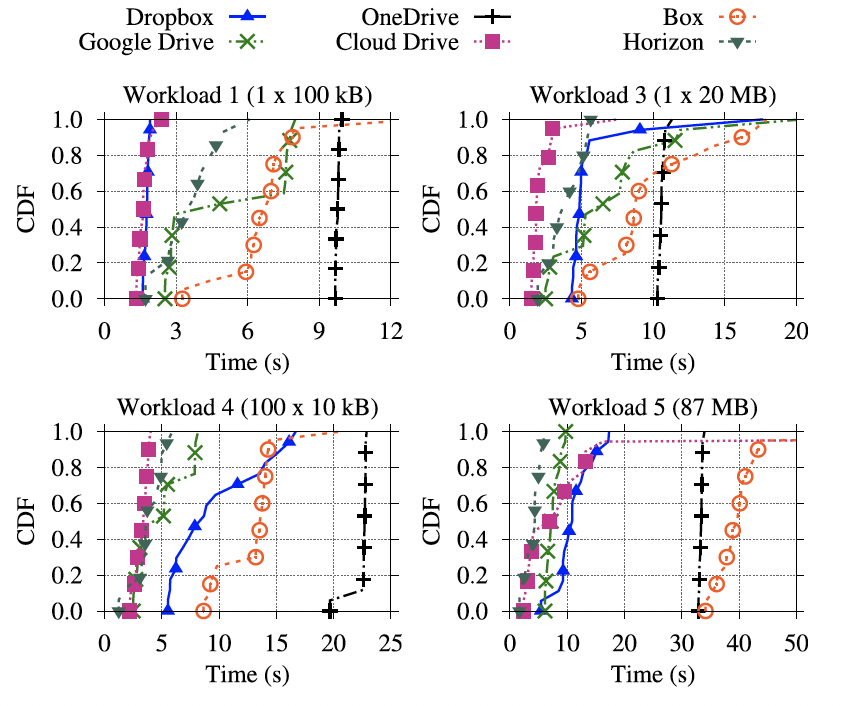
\includegraphics[scale=0.7]{images/start_up_delay}
        \caption{\label{fig:synchronization start up}Start up delays}
    \end{figure}

    \item[\textbf{Upload and Download Duration}] for single-file workloads across all 3 services are determined primarily by data center placements and system parameters. When multiple files are uploaded, though, each client's capabilities and other factors are much more significant. Once again, Dropbox wins both workloads involving multiple files thanks to its bundling implementation by a huge margin in one case, with the trade-off of having higher start up delay as mentioned earlier. The next best performer is Google Drive, with mostly comparable results to that of Dropbox. Box, however, is by far the worst of the 3, with workload 5 taking and absurd amount of time by comparison, leaving lots of room for improvement. All results are visible in \autoref{fig:upload}

    \begin{figure} [h]
        \centering
        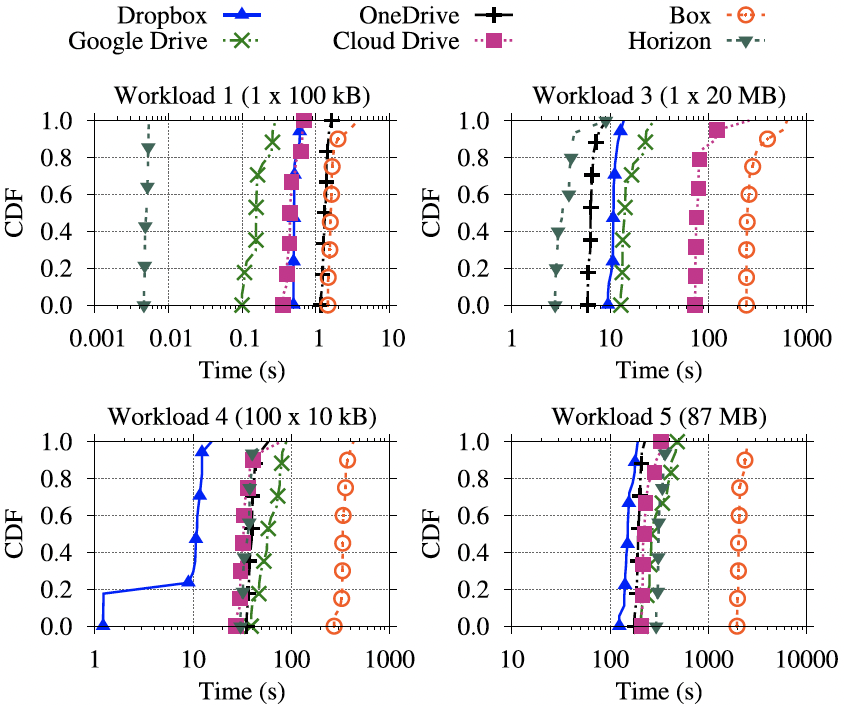
\includegraphics[scale=0.7]{images/upload_times}
        \caption{\label{fig:upload}Upload times}
    \end{figure}

    \item[\textbf{Propagation Delay}], computed as the difference between the download and upload starting times,  does not exhibit much variation, with all services waiting roughly the same time before starting the download, with the exception of workload 3 as shown in \autoref{fig:propagation delay}, where Box again falls significantly behind the other two services.

    \begin{figure} [h]
        \centering
        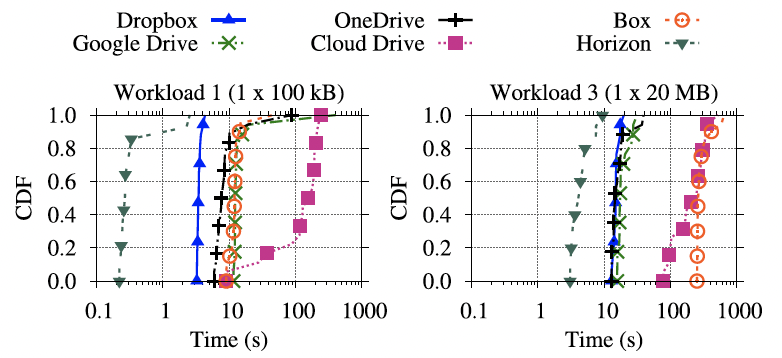
\includegraphics[scale=0.7]{images/propagation_delay}
        \caption{\label{fig:propagation delay}Propagation delays}
    \end{figure}

    \item[\textbf{Traffic Overhead}] is calculated by dividing total exchanged traffic over twice the total file size. For synchronizing single small files, the total overhead is significant for all services, even Dropbox, probably due to implementing its advanced capabilities. This is one case, however, where Box is the winner, likely for the opposite reason, that is, it is lacking most advanced capabilities. In addition, as large files are submitted, the overhead decreased dramatically, though Dropbox still exhibits a significant overhead of around 7\%. The situation changes, however, when many small files are synchronized, in which case bundling plays an essential role. Since Dropbox is the only service that bundles files, the total overhead it produces is significantly less than the other two services, which have approximately the same overhead even though Google Drive uses compression (see \autoref{fig:traffic overhead}). Indeed, it is the lack of bundling, and hence the need for several TCP/SSL connections, that introduces this additional overhead.

    \begin{figure} [h]
        \centering
        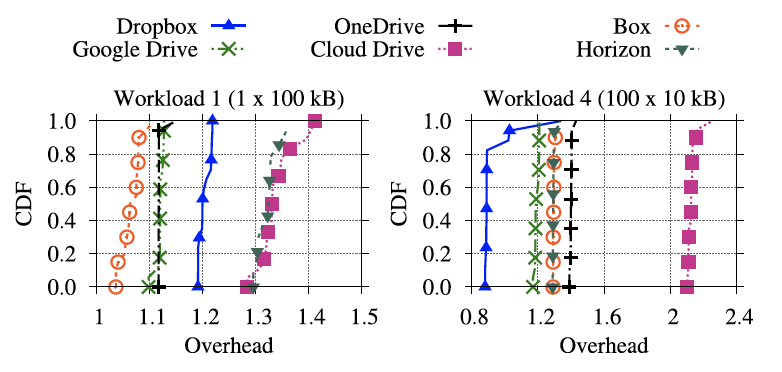
\includegraphics[scale=0.7]{images/traffic_overhead}
        \caption{\label{fig:traffic overhead}Traffic overhead}
    \end{figure}

\end{description}

\section{Conclusions}
Overall, both of the object storage services investigated (S3 and Blob Storage) are very similar in some aspects, and yet quite different in others. Specifically, they both provide functionality to make storage management more convenient, as they allow key-value pairs to be attached to objects (S3 object tags and blob index tags) and inventory reports to be generated, providing an overview of the user's stored data. Both services also support the monitoring and logging of resource usage, however S3 is more sophisticated in this regard, providing organization-level insight into storage access patterns via S3 Storage Lens, and making recommendations for when storage class transitions should be made via S3 Storage Class Analysis. When it comes to storage classes, even though both S3 and Blob Storage feature a variety of storage classes to suit different access patterns, only S3 has classes that allow automatic transition to different access tiers when it is cost-efficient (S3 Intelligent-Tiering) , and also allow for on-site data storage (S3 Outposts). On the other hand, Blob Storage lacks these options and its archival tier has certain limitations, as not all accounts can make use of it. To enforce data redundancy,  both services support data replication, even across different regions, but neither one can be considered the better option. To illustrate, while Blob Storage promises better durability via the Service-level agreement (SLA) compared to S3 (16 9's vs 11 9's of durability), blob's redundancy settings are account-wide, while S3 allows for even object-level specification and has a SLA backing replication speed with S3 Replication Time Control. Such differences are not present in the Availability SLAs of these services, though, as they both promise similar availability (specified with monthly uptime percentage), with the main differences being that Blob Storage specifies availability for reads and writes, while S3 offers full (100\% Service Credit) compensation if availability is significantly low. Furthermore, for security, the two services support both client-side and server-side encryption for data in transit (along with enforcement of HTTPS /TLS) and for data at rest, with blob having an advantage with double encryption (encryption at the service and infrastructure level) and a potential disadvantage if the two storage account keys aren't properly managed. A variety of access control mechanisms are also made available by both services, and they are equally strong, with the only exception being that Blob Storage does not support resource-based access policies. Also comparable are the options that are offered to protect and recover from accidental data deletions and modifications, with both services allowing for different versions of objects/blobs to be maintained and locks to be placed at various levels, thus preventing data modifications. Performance-wise, there are no significant differences in latency between the services however, regarding throughput, S3 performs better for large files ($>=$100MB), while Blob Storage is more capable for smaller files. Additionally, though upload speeds are stable for both services, download speeds with certain S3 servers in particular were not consistent whatsoever, while connection overhead was found to be much higher when using Blob Storage, due to the establishment of separate connections for each file upload.  Both services apply a "pay-as-you-go" payment model and, from the sample that we gathered, prices are comparable for similar access tiers, but Blob seems to charge 25\% less than expected. 

Many similarities and differences were also observed after comparing three popular file storage providers (Dropbox, Box and Google Drive). All services offer a variety of pricing plans to customers, ranging from very expensive custom plans to free, albeit limited, plans. Box was found to be the most expensive of the three overall, but it did not limit storage space for most of its plans, while Google Drive's plans were the most cost-efficient, as they include all Google Workspace applications. Google Drive was also found to be the most scalable service, allowing files of up to 5 TB to be uploaded at a time, compared to the 2 TB and 150 GB limit of Dropbox and Box, respectively, but all of them supported every file type along with unlimited users, storage and devices with at least one of their offered plans.  File sharing, which is one of the primary benefits of file storage, is supported by the three services via shared links which can be sent to anyone, customized with specific access permissions, expiration dates etc. for secure sharing.  In this aspect, only Google Drive was found lacking, as it provides no way to gather files from various people.  Real-time collaboration is also facilitated , as each service has its own collaboration solution (Dropbox Paper, Box Notes, Google Docs), where users can preview and work on all kinds of files  (e.g., text and video), make comments, and assign tasks. Of the three, Dropbox Paper is the most sophisticated, allowing annotations to be made even on videos, whereas Google Docs does not provide nearly as much flexibility when embedding and annotating media. All services integrate with many third-party apps like Zoom or Slack, enhancing productivity. With regard to security and data protection, each of the services uses sophisticated encryption for data both in transit and at rest, with Google Drive also supporting encryption at the client-side, while each service maintains a large number of file version to revert back if needed. Furthermore, all services provide strong admin controls (generate audit logs, view alerts etc.), mechanisms for controlling which devices can access data based on password, minimum OS , location and other requirements, along with malware detection. Dropbox Vault  and Box Zones are features unique to those services, with the former providing an extra secure PIN-protected folder, and the latter allowing data protection and privacy compliance requirements to be met by allowing customers to specify in which region the data should be stored. To optimize performance, the services make use of certain client capabilities such as bundling, chunking, and delta encoding. Dropbox is the service with the largest amount of implemented capabilities, whereas Box only implements chunking, and its performance suffers as a result. Specifically, Dropbox is the best-performing when it came to synchronization start up of small files and upload/download duration, while Box was consistently the slowest, except for traffic overhead of small files, where it performed the best due to having no advanced capabilities. In all other cases, Dropbox and Google Drive performed comparably well. 
